%!TEX root = ../main.tex
\chapter{Monte Carlo Estimation of the Density of the Sum of Dependent Random Variables}

\section{Introduction}

Sums of random variables are fundamental to modeling stochastic phenomena. In finance, risk managers need to predict the distribution of a portfolio's future value which is the sum of multiple assets; similarly, the distribution of the sum of an individual asset's returns over time is needed for valuation of some exotic (e.g.\ Asian) options \cite{mcneil2015quantitative,ruschendorf2013mathematical}. In insurance, the probability of ruin (i.e.\ bankruptcy) is determined by the distribution of aggregate losses (sums of individual claims of random size) \cite{klugman2012loss,asmussen2010ruin}. Lastly, wireless system engineers model total interference in a wireless communications network as the sum of all interfering signals (often lognormally distributed) \cite{fischione2007approximation}. 

In this article, we consider estimating the probability density function (pdf) of sums of random variables (rvs). A major motivation for obtaining accurate pdf estimates of a rv is to produce confidence intervals for quantiles. For example, the US Nuclear Regulatory Commission specifies regulations in terms of the ``95/95'' rule, i.e.\ the upper 95\% confidence interval for a 95\% quantile.  The most common approach  \cite{asmussen2017conditional}  is to first  estimate the cumulative distribution function (cdf) via
\[ \widehat{F}_X(x) = \frac1R \sum_{r=1}^R \ind{ X^{[r]} \le x} \quad \text{for } X^{[1]}, \dots, X^{[R]} \iidDist F_X \,, \]
and then the quantile  $\widehat{q}_\alpha=  \widehat{F}_X^{-1}(\alpha)$. In the obvious notation, we then have the convergence in distribution:
\[ 
\sqrt{R} (\widehat{q}_\alpha - q_\alpha) \stackrel{\mathcal{D}}{\longrightarrow} {\sf N}\left(0, \frac{\alpha(1-\alpha)}{f_X(q_\alpha)^2}\right)  \quad \text{ as } R \to \infty,
\]
where the limiting variance depends on the unknown density $f_X(q_\alpha)$.  Thus, any confidence intervals for $\widehat{q}_\alpha$ require estimation of the density $f_X(q_\alpha)$, which is a highly nontrivial problem.


In general, the pdf of a sum of rvs is only available via an $n$-dimensional convolution.
The convolution  cannot be computed  analytically  or numerically (via quadrature), except in the special cases of normal or exponential rvs. For this reason, one has to resort to density estimation methods such as kernel density estimation \cite{botev2010kernel}, Conditional Monte Carlo \cite{asmussen2017conditional}, or a modification of the Asmussen--Kroese estimator \cite{Asmussen2006}. 


The purpose of this work is to  present a novel Monte Carlo estimator of the pdf of the sum of (in)dependent  rvs. There are three main  advantages of the proposed estimator. First,
we show that the estimator often enjoys smaller variance than its competitors.
Second,  the estimator only requires  evaluation of   the joint pdf up 
to an (typically unknown) normalizing constant, a situation similar to the application of Markov chain Monte Carlo. As a result of this, the estimator is useful in estimating posterior marginal densities in Bayesian inference (Section~\ref{ssec:Marginals}).  Finally, when the rvs have a copula dependence, the proposed estimator is simpler to implement than its Conditional Monte Carlo counterpart (Section~\ref{ssec:CondMC}). 
Note that the source code used in this paper is available online \cite{Code}.




Throughout the paper, we use lowercase boldface letters like $\v{c}$, $\v{x}$, $\v{y}$ for non-random vectors and uppercase boldface letters like $\v{X}$ for random vectors, and $\v{1}$ for the vector of 1's. If $\v{X}$ is of length $n$, we write:  $\v{X}=(X_1, \dots, X_n)^\top$. The inner-product is denoted  $\v{x} \cdot \v{y}$. For a differentiable  function $f: \bb R^n\mapsto \bb R$, we write
\[ \nabla f(\v{z}) = \left. \left( \partial f(\v{x}) / \partial x_1 , \dots, \partial f(\v{x}) / \partial x_n \right)^\top \right\vert_{\v{x} = \v{z}}, \] 
and use $\nabla_i f(\v{z})$ to denote the $i$'th component of $\nabla f(\v{z})$. 


\section{Proposed Push--Out Estimator} \label{sec:GeneralSetup}
Our method is derived from the ``Push-Out'' method \cite{RubinsteinReuven1992Saod,kroese2007solutions} in  sensitivity analysis of Discrete Event Systems, where a judiciously chosen change of variable  allows differentiation of an otherwise non-
smooth function. We thus tackle the pdf estimation problem by 
viewing it as a special type of  sensitivity analysis. We note 
that a similar insight was used in  Example 5.7 of \cite{
asmussen2007stochastic}, but that estimator is strictly 
restricted to iid sums of positive random variables, with the 
further requirement that the pdf $f_X(0) > 0$. This positivity 
condition is quite restrictive ---  it excludes cases such as 
Pareto rvs or  Weibull rvs with shape parameter greater than 
one. As we shall see, none of these restrictions apply to our  
estimator.




\begin{assumption} \label{assumption}
The random vector $\v{X}$ has a density $f_{\v{X}}$  (each $X_i$ is supported either on the entire real line or a half-real line), the gradient $\nabla f_{\v{X}}$ is a continuous function on the  support of $\v{X}$, and we have the integrability condition
$
\bb E\left|\v X \cdot \nabla \log f_{\v{X}}(\v X)\right|<\infty 
$ (here $\v X\sim F_{\v X}$). \hfill $\Diamond$
\end{assumption}
The proposed estimator is based on the following  simple formulas, proved in the appendix. 
\begin{proposition} \label{prop:DensityRepresentation}
For the rv $S = \sum_{i=1}^n X_i = \v{1} \cdot \v{X}$ where $\v{X}$ satisfies Assumption~\ref{assumption},
\begin{align} \label{Pushout}
f_S(s) &= \hphantom{-} \frac{1}{s} \Exp \big\{ \ind{\v{1} \cdot \v{X} \le s} [ \v X \cdot \nabla \log f_{\v{X}}(\v X) + n ] \big\} 
% \label{eq:RTexp} 
% &= -\frac{1}{s} \Exp \big\{ \ind{\v{1} \cdot \v{X} > s} [ \v X \cdot \nabla \log f_{\v{X}}(\v X) + n ] \big\} \,
\end{align}
for any $s \not= 0$. \hfill $\Diamond$
\end{proposition}


\begin{corollary} \label{cor:WeightedSums}
For the rv $S = \sum_{i=1}^n c_i X_i = \v{c} \cdot \v{X}$
where $\v{X}$ satisfies Assumption~\ref{assumption}, 
\begin{align} \label{PushoutWeighted}
f_S(s)
&= \hphantom{-} \frac{1}{s} \Exp \big\{ \ind{\v{c} \cdot \v{X} \le s} [ \v{X} \cdot \nabla \log f_{\v{X}}(\v{X}) + n ] \big\} 
% &= -\frac{1}{s} \Exp \big\{ \ind{\v{c} \cdot \v{X} > s} [ \v{X} \cdot \nabla \log f_{\v{X}}(\v{X}) + n ] \big\} 
\end{align}
for any $s \not= 0$, and where each $c_i \not=0$. \hfill $\Diamond$
\end{corollary}

More generally, for rvs of the form $S = \sum_{i=1}^n h_i(X_i)$, where each $h_i$ is invertible on its support, and the transformed random variables $h(X_i)$ each obey Assumption \ref{assumption}, we have that
\begin{equation} \label{PushoutGeneral} 
\textstyle
f(s) = \hphantom{-} \frac{1}{s} \Exp\big\{ \ind{S \le s} [ \frac{\v h(\v X)}{\v h'(\v X)} \cdot \nabla \log f_{\v X}(\v X) + \v{1} \cdot \nabla \frac{\v h(\v X)}{\v h'(\v X)} ] \big\} \,. 
\end{equation}
Since the more general  case \eqref{PushoutGeneral} is, after some rearrangement, equivalent to the simpler one  \eqref{Pushout},  we henceforth only consider  sums of the form $S = \sum_{i=1}^n X_i$.



It is straightforward to show that \eqref{Pushout}, \eqref{PushoutWeighted}, \eqref{PushoutGeneral} still hold if the indicators $\ind{\cdot}$ are replaced by $-(1-\ind{\cdot})$. This  suggests the pair of  (unbiased)  estimators ($\v X \sim F_{\v X}$):
\[
\begin{split}
\widehat{f}_{1}(s)& = \hphantom{-} \frac{1}{s} \ind{\v{1} \cdot \v{X} \le s} \big[ \v X \cdot \nabla \log f_{\v{X}}\big(\v X\big) + n \big] \\
\widehat{f}_{2}(s)& = -\frac{1}{s} \ind{\v{1} \cdot \v{X} > s} \big[ \v X \cdot \nabla \log f_{\v{X}}\big(\v X\big) + n \big] 
\end{split}
\]
A weighted combination of  the latter two yields our  proposed ``push-out'' estimator:
\begin{equation} \label{MixtureEstimator}
\widehat{f}(s ; p) = p \widehat{f}_{1}(s) + (1-p) \widehat{f}_{2}(s),
\end{equation}
where $p \in \bb R$ is chosen to (approximately) minimize the overall variance, as follows.

Let $\Sigma$ be the sample covariance matrix of $(\widehat{f}_1,\widehat{f}_2)$ and note that 
\[
\widehat{\Var}(p)= (\Sigma_{11} + \Sigma_{22} - 2 \Sigma_{12}) \, p^2 + 2(\Sigma_{12} - \Sigma_{22})\, p + \Sigma_{22}
\]
is an unbiased estimator of the variance of (\ref{MixtureEstimator}). Then, we chose $p$ to be 
\begin{equation} \label{MixtureCoefficient}
p^\star = \argmin_p \widehat{\Var}(p) = (\Sigma_{22} - \Sigma_{12})/(\Sigma_{11} + \Sigma_{22} - 2 \Sigma_{12}).
\end{equation}
In order to ensure the unbiasedness of \eqref{MixtureEstimator}, we may, for example, estimate  $p^\star$   from a pilot (independent) sample, as explained in Section~\ref{sec:NumericalResults}. 

We note that a downside of our push-out estimator is that the integrability condition in Assumption~\ref{assumption} is difficult to verify in many practical settings. As a matter of fact, in our simulations in Section~\ref{sec:NumericalResults} we implicitly assume without verifying the  stronger condition  $\bb E\left|\v X \cdot \nabla \log f_{\v{X}}(\v X)\right|^4<\infty$, which not only ensures the finite variance of the push-out estimator \eqref{MixtureEstimator}, but also the reliability of its sample (empirical) variance estimator (the variance of the sample variance has to be finite).

\section{Competitor Methods} 
In the following Sections~\ref{ssec:CondMC} and \ref{ssec:AK} we describe our main competitors --- the Conditional Monte Carlo  and Asmussen--Kroese estimators \cite{asmussen2017conditional}. We then use these methods as benchmarks to illustrate the performance of the proposed estimator in various settings. 

\subsection{Conditional Monte Carlo estimator} \label{ssec:CondMC}

The Conditional Monte Carlo estimator \cite{asmussen2017conditional} takes the form
\[ \widehat{f}_{\mathrm{Cond}}(s) = \frac1n \sum_{i=1}^n f_{X_i | \v{X}_{-i}}( s - S_{-i} ) , \quad \v{X} \sim F_{\v{X}},
 \]
where the notation $\v{X}_{-i}$ denotes the vector $\v{X}$ with the $i$-th component removed and $S_{-i}=\v 1 \cdot \v X_{-i}$. This is particularly simple for the independent case, as $f_{X_i | \v{X}_{-i}} = f_{X_i}$.
% \[ \widehat{f}_{\mathrm{Cond}}(s) = \frac1n \sum_{i=1}^n f_{X_i}( s - \v{1}\cdot\v{X}_{-i} ) , \quad \v{X} \sim F_{\v{X}} \,. \]

We now examine the dependent case where $\v{X}$'s dependence structure is given by an Archimedean copula with generator $\psi$; i.e., the cdf yields
\begin{equation*}  
\textstyle
\Prob(X_1\le F_{X_1}^{-1}(u_1), \dots, X_n \le F_{X_n}^{-1}(u_n)) =\phi\big( \sum_{i=1}^n \psi(u_i) \big),\quad \v u\in[0,1]^n,
\end{equation*}
where $\phi\equiv \psi^{-1}$ is the functional inverse of $\psi$.
 The  conditional densities of $\v X$ can be calculated from the formula 
($\phi^{(n)}$ denotes $n$-th derivative)
\begin{equation} \label{GenCondMC}
f_{X_i | \v{X}_{-i}}(x_i | \v{x}_{-i}) = f_{X_i}(x_i) \psi^{(1)}( F_{X_i}(x_i)) \frac{\phi^{(n)}( \sum_{j=1}^n \psi(F_{X_j}(x_j)) ) }{\phi^{(n-1)}( \sum_{j\not=i} \psi(F_{X_j}(x_j)))} \,.
\end{equation}

Some Archimedean copulas, such as the Clayton and Gumbel--Hougaard copulas, have what is called a Marshall--Olkin representation. An Archimedean copula is in the Marshall--Olkin representation class if  $\phi(s) = \Exp[\e^{-s Z}]$ for some positive rv $Z$ with cdf $F_Z$. Then an $\v X$ with this dependence structure can be simulated via
\begin{equation} \label{MarshallOlkin} \v{X} = \Big(F_{X_1}^{-1}\Big( \phi\Big(\frac{E_1}{Z}\Big) \Big), \dots, F_{X_n}^{-1}\Big( \phi\Big(\frac{E_n}{Z}\Big) \Big) \Big) , \quad E_i \iidDist \mathsf{Exp}(1),\; Z \sim F_Z \,.
\end{equation}
For this case, Asmussen \cite[Proposition~8.3]{asmussen2017conditional} conditions upon the $Z$ as well as $\v{X}_{-i}$ to obtain what we call the \emph{extended Conditional Monte Carlo estimator}
\begin{align} \label{ExtCondMC}
 \widehat{f}_{\mathrm{ExtCond}}(s) &= \frac{1}{n}\sum_{i=1}^n f_{X_i | \v{X}_{-i}, Z}( s - S_{-i} ),  
\end{align}
where $f_{X_i | \v{X}_{-i}, Z}(x_i ) = -z \psi'(F_i( x_i )) f_{X_i}( x_i ) \, \e^{ -z \psi(F_i( x_i )) }$ and  $\v{X}$ is given by \eqref{MarshallOlkin}.


We will use this estimator as a benchmark in our comparisons later on.

\subsection{Asmussen--Kroese estimator} \label{ssec:AK}

The Asmussen--Kroese estimator \cite{Asmussen2006} (typically for tail probabilities) is defined as 
\[
\widehat{F}_{\mathrm{AK}}(s) = 1 - \sum_{i=1}^n 
\overline{F}_{X_i | \v{X}_{-i}}( \max\{ M_{-i}, s - S_{-i} \} ) \]
where: $M_{-i} = \max\{ X_1,\ldots,X_{i-1},X_{i+1},\ldots,X_n\}$  and  $\overline{F}_{X_i | \v{X}_{-i}}(x)=1-F_{X_i | \v{X}_{-i}}(x)$.
Each $\overline{F}_{X_i | \v{X}_{-i}}( \max\{ M_{-i}, s - S_{-i} \} )=
\overline{F}_{X_i | \v{X}_{-i}}( s - S_{-i})$,
whenever $M_{-i}+S_{-i}<s$. Thus,
we can take the derivative of this  piecewise  estimator to obtain
\[
\widehat{f}_{\mathrm{AK}}(s) = \sum_{i=1}^n 
f_{X_i | \v{X}_{-i}}( s - S_{-i} ) \ind{M_{-i} + S_{-i} \le s }, \]
which can be viewed as alternative conditional estimator.
When it is applicable, we use the ``extended'' form of this estimator where $f_{X_i | \v{X}_{-i}}$ is replaced with $f_{X_i | \v{X}_{-i}, Z}$ as in Section~\ref{ssec:CondMC}. Notice that the term  $1/n$ in \eqref{ExtCondMC} does not appear here. 

\section{Numerical Experiments and Extensions to Marginal Distributions} \label{sec:NumericalResults}

In Section~\ref{ssec:CopulaExamples}, for various distributions of $\v{X}$ we compare: i) our proposed method, ii) the conditional MC estimator, iii) the Asmussen--Kroese (AK) estimator, and iv) the default kernel-density estimator (KDE) in \textsc{Mathematica}. Following this, Section~\ref{ssec:Marginals} extends the estimator to the case of marginal density estimation in the context of Bayesian statistics. 

\subsection{Copula examples} \label{ssec:CopulaExamples}

When the Marshall--Olkin representation \eqref{MarshallOlkin} is available, we simulate $\v{X}$ using this form and give results for the extended version \eqref{ExtCondMC} of the conditional MC estimator. If this representation is unavailable, we use the standard version \eqref{GenCondMC} of the conditional MC estimator where $\v{X}$ is sampled using \textsc{Mathematica}'s built-in routines (to replicate this in another language one could simulate $\v{X}$ using the  ``conditional distribution method'' \cite[p.~41]{nelsen2006introduction}). KDE is provided by \textsc{Mathematica}'s {\sf KernelMixtureDistribution} function with default bandwidth; to keep the support positive, we reflect this estimator about the origin. We report on all distributions and copulas as they are parametrized in \textsc{Mathematica}. 
 
We conduct 4 experiments, each one depicted on  Figures~1 to 4 below. 
Each experiment uses $R=10^5$ iid replicates of $\v{X}$ which are common to all estimators (our estimator uses the first 5\% of these to obtain the $p^\star$ coefficient, as in \eqref{MixtureCoefficient}, and the remaining samples for pdf estimation as in (\ref{MixtureEstimator})). 

Our primary measure of performance is  (square root of) the \emph{work-normalized relative variance}: 
\[\textstyle
 \text{WNRV}(\widehat{f}(x)) = \text{(CPU\_Time)} \times \Var( \widehat{f}(x) ) / (R[\widehat{f}(x)]^2)
\]  
 For each experiment we also display a subplot of the estimated density function, as well as the estimated standard deviation. 

Figures 1--4 show that our proposed estimator consistently has the smallest WNRV. In Figures 3 and 4, it also has the smallest standard deviation. In Figure~1, the simple case for the sum of iid gamma rvs, the standard deviation of our estimator is similar to the Conditional MC method. In Figure~2, the sum of non-identical lognormal variables under a Frank copula, the AK estimator has the smallest standard deviation (it was designed for such subexponential distributions). In general, the Conditional MC method does not perform well in the case of heavy-tailed summands, as in Figures 2 and 3. 

     
    \begin{figure}[H]
		\caption{Sum of $n=40$ iid $\mathsf{Gamma}(3,2)$ random variables.}
    \centering
    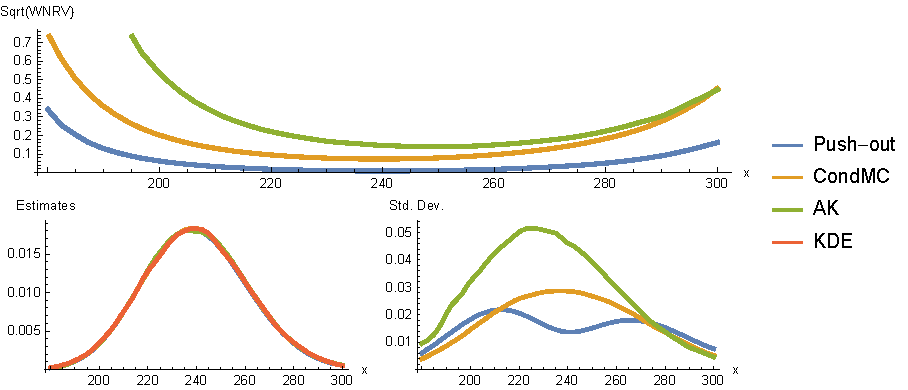
\includegraphics[width=\textwidth]{Independent_Gamma_40_dim.pdf}\vspace{3mm}
	\end{figure}



 \begin{figure}[H]
		\caption{    Sum of $n=10$ random variables where $X_i \sim \mathsf{Lognormal}(i-10,\sqrt{i})$ with a $\mathsf{Frank}(1/1000)$ copula. The choice of marginals mimic the challenging (and somewhat pathological) example considered in \cite{asmussen2011efficient}.}\vspace{5mm}
    \centering
    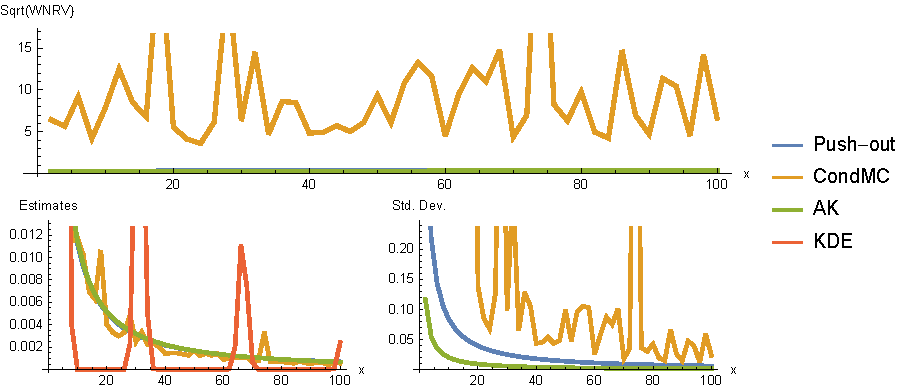
\includegraphics[width=\textwidth]{Frank_LogNormal_10_dim.pdf}\vspace{3mm}
    \end{figure}


 

    \begin{figure}[H]
				\caption{    Sum of $n=10$ $\mathsf{Weibull}(0.3, 1)$ random variables with a $\mathsf{Clayton}(1/5)$ copula.}\vspace{3mm}
    \centering
    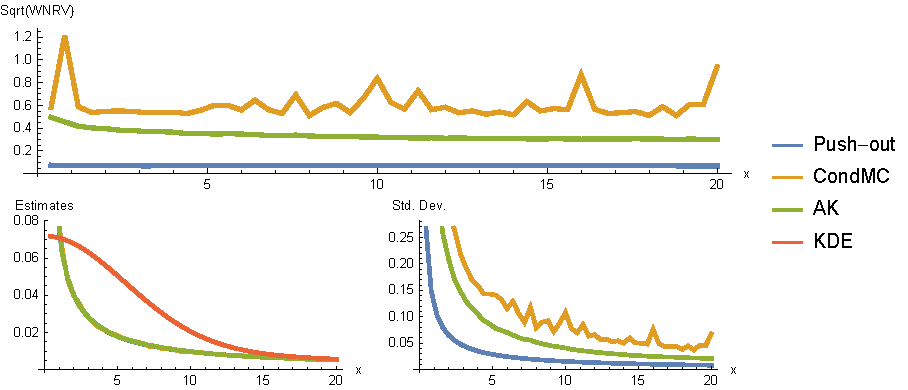
\includegraphics[width=\textwidth]{Clayton_Weibull_10_dim.pdf}
		\label{Test:Clayton}
    \end{figure}



   \begin{figure}[H]
			\caption{Sum of $n=15$ $\mathsf{Exp}(1)$ random variables with a $\mathsf{GumbelHougaard}(5)$ copula.}\vspace{3mm}
    \centering
    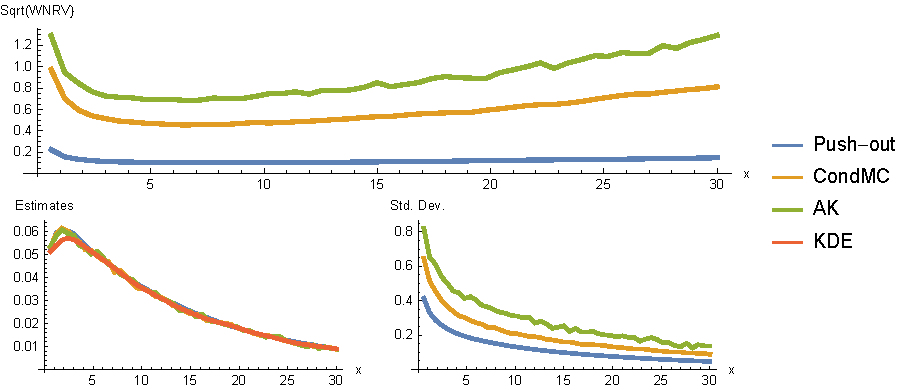
\includegraphics[width=\textwidth]{GumbelHougaard_Exponential_15_dim.pdf}
    \end{figure}

It is important to note that due to the $1/s$ term, the proposed push-out estimator can have large variance for very small $s$, even when $F(s)$ or $1 - F(s)$ is not  close to zero. This problem can be resolved with a simple linear shift, as follows.  If one element, say $X_1$, is supported on $\bb{R}$, then $f_S(s) = f_{\widetilde{S}}(s-a)$ for $a \in \mathbb{R}$, where $\widetilde{S} = (X_1+a) + X_2 + \dots + X_n$.  We can then use the original estimator (with shifted values of $s$ and $X_1$) to obtain estimates of the  density of $S$ near or at zero.  



\subsection{Estimating Marginal Distributions with Bayesian Applications} \label{ssec:Marginals}
One  extension of the estimator is in the estimation of marginal densities.

\begin{proposition} \label{lemma:MarginalDensity}
    For an $\v{X}$ which satisfies Assumption~\ref{assumption}, the marginal densities are given by
    \begin{equation} \label{MarginalExp}
    f_{X_i}(s) = \frac1s \Exp \big\{ \ind{ X_i \le s}  \big(X_i \nabla_i \log f_{\v X}(\v{X}) + 1 \big)  \big\}
    \end{equation}
    for $i=1,\dots,n$, and $s \not=0$. \hfill $\Diamond$
    \end{proposition}
We use the weighted estimator of the form \eqref{MixtureEstimator} which is based on \eqref{MarginalExp}. A nice feature of the corresponding estimator is that, due to the presence of the $\nabla \log f_{\v X}(\v x)$ term,  the normalizing constant of $f$ need not be known. 



As an example, we use Markov Chain Monte Carlo to obtain samples from the posterior density of a Bayesian model, and use these to estimate the posterior marginal pdfs with our push-out estimator.

 We consider the well-known ``Pima Indians'' dataset (standardized), which records a binary response variable  (the incidence of diabetes) for $532$ women, along with seven possible predictors. We specify a Logistic Regression model with predictors: {\em Number of Pregnancies}, {\em Plasma Glucose Concentration}, {\em Body Mass Index}, {\em Diabetes Pedigree Function}, and {\em Age} (see \cite{Friel2012} for justification). The prior is $\v \beta \sim {\sf N}(\v 0, \m I)$, as in \cite{Friel2012}. 

To obtain samples from the posterior density, we implement an isotropic Random Walk sampler, using a radially symmetric Gaussian density with $\sigma^2 = 7.5\times 10^{-3}$ (trace plots indicate this choice mixes well for the model). We note that by introducing 
auxiliary random variables, it is possible to simulate from this Bayesian posterior  using a complicated Gibbs sampler  \cite[Equation 8]{holmes2006bayesian}, which requires simulation of costly (non-standard) \emph{Kolmogorov-Smirnov}-distributed random variables, and truncated normal and truncated logistic random variables.  In contrast, the Random Walk sampler is simpler to implement. 



We ran the Random Walk sampler for $10^3$ steps for burn-in, then used the next $5 \times 10^4$ samples (without any thinning) to obtain a KDE, as well as density estimates using our push-out estimator.  As a benchmark, we  compare the accuracy with a KDE constructed using every $50$-th  sample from an MCMC chain of length $50\times 5 \times 10^6$. 




The result of this comparison is depicted on Figure~\ref{fig:marginal} below.
\begin{figure}[H]
    \centering 
    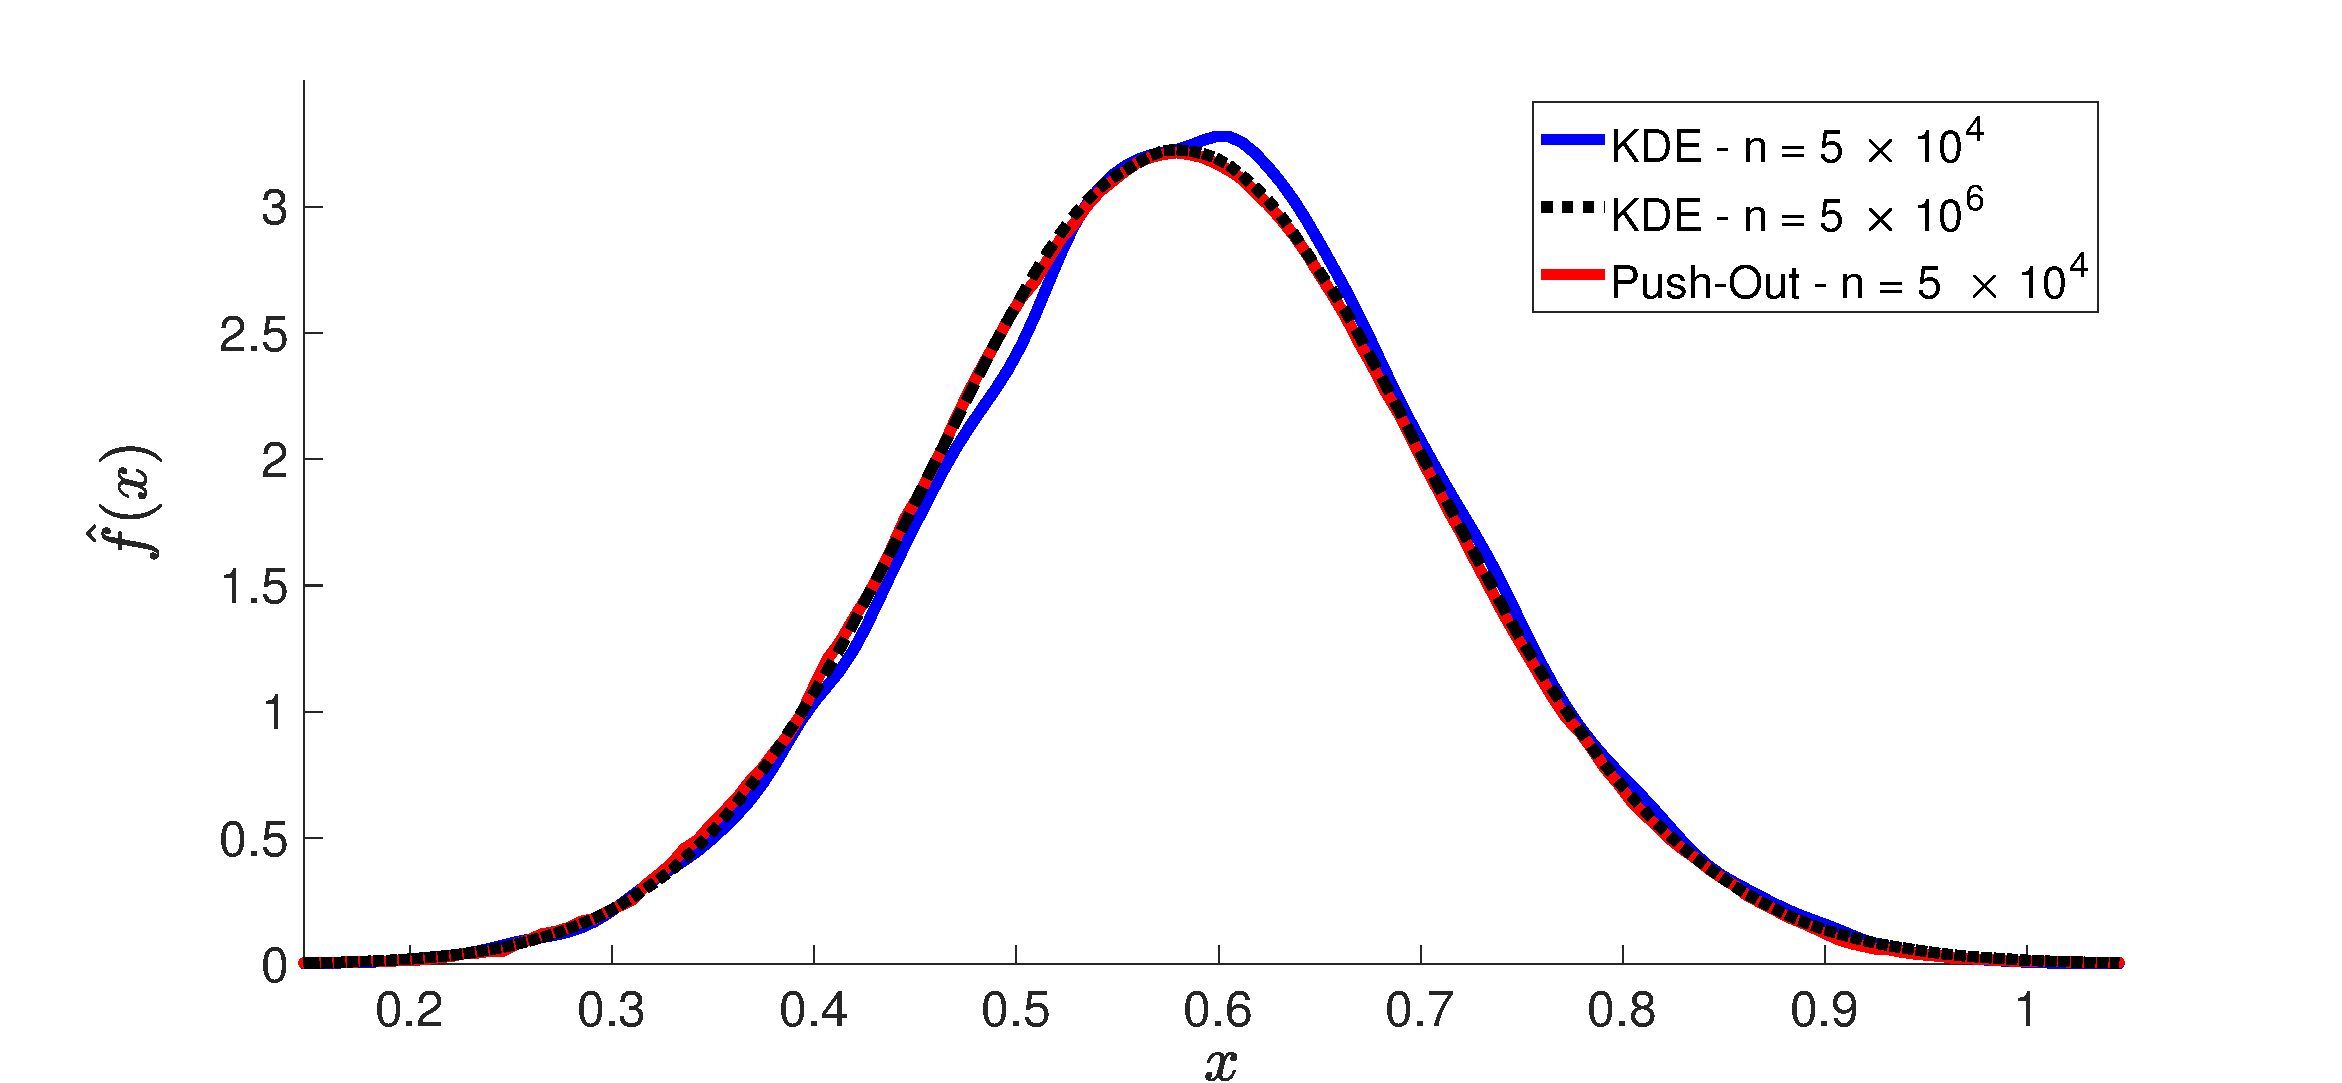
\includegraphics[width=1\textwidth]{pima.pdf}
    \caption{Density estimation of posterior marginal corresponding to the coefficient parameter of the {\em Body Mass Index} predictor variable.}
    \label{fig:marginal}
\end{figure}



As expected, using the same set of samples, the push-out estimator yields a  more accurate estimate than KDE. The reason for the lower accuracy of KDE  in this context is well-known --- a mean square error convergence of
$\c O(n^{-4/5})$, instead of the canonical Monte Carlo rate of $\c O(1/n)$,
due to the presence of non-negligible bias in the KDE estimator (see \cite{botev2010kernel}, for example).



\subsection{Discussion} \label{sec:Discussion}
In our experiments, the proposed push-out estimator is usually as accurate, or more accurate, than the Conditional MC and AK estimators. However, when computing time is taken into account, then our push-out estimator truly excels.  For example, in the test with the Clayton copula on Figure~\ref{Test:Clayton}, our proposed estimator took 3.03 minutes to compute, whereas the extended Conditional MC estimator took 9.16 minutes, and the Asmussen--Kroese estimator took 9.81 minutes
(for source code see \cite{Code}). One reason for this lower computing cost is that evaluation of the gradient of the joint log-pdf, $\nabla \log f_{\v{X}}$, is often much faster than evaluation of the conditional pdfs $f_{X_i | \v{X}_{-i}}$.  

A practical difficulty with the extended Conditional MC estimator \eqref{ExtCondMC} is the simulation of the auxiliary variable $Z$.
For example, simulation is difficult and time-consuming for the $\mathsf{GumbelHougaard}(\theta)$ copula with generator $\psi(u) = [-\log( u )]^\theta$, because in that case  $Z \sim \mathsf{Stable}(1, \theta^{-1}, 1, 0, \cos(\frac{\pi}{2 \theta})^\theta)$ is a complicated L\'evy $\alpha$-stable distribution. (On the other hand, simulation is simple for the $\mathsf{Clayton}(\theta)$ copula with generator $\psi(u) = \theta (u^{-1/\theta} - 1)$, because  $Z \sim \mathsf{Gamma}(\theta, 1/\theta)$.) It is also worth noting that many Archimedean copulas, e.g. Frank copula, do not have a Marshall--Olkin representation.

We also remark that one must be cautious with the reported estimate of estimator variance when using Conditional Monte Carlo. In heavy-tailed settings, the estimator has large variance, as illustrated using a sum of 30 iid Weibull rvs on Figure~\ref{fig:weibull}.



 \begin{figure}[htb]
    \centering 
    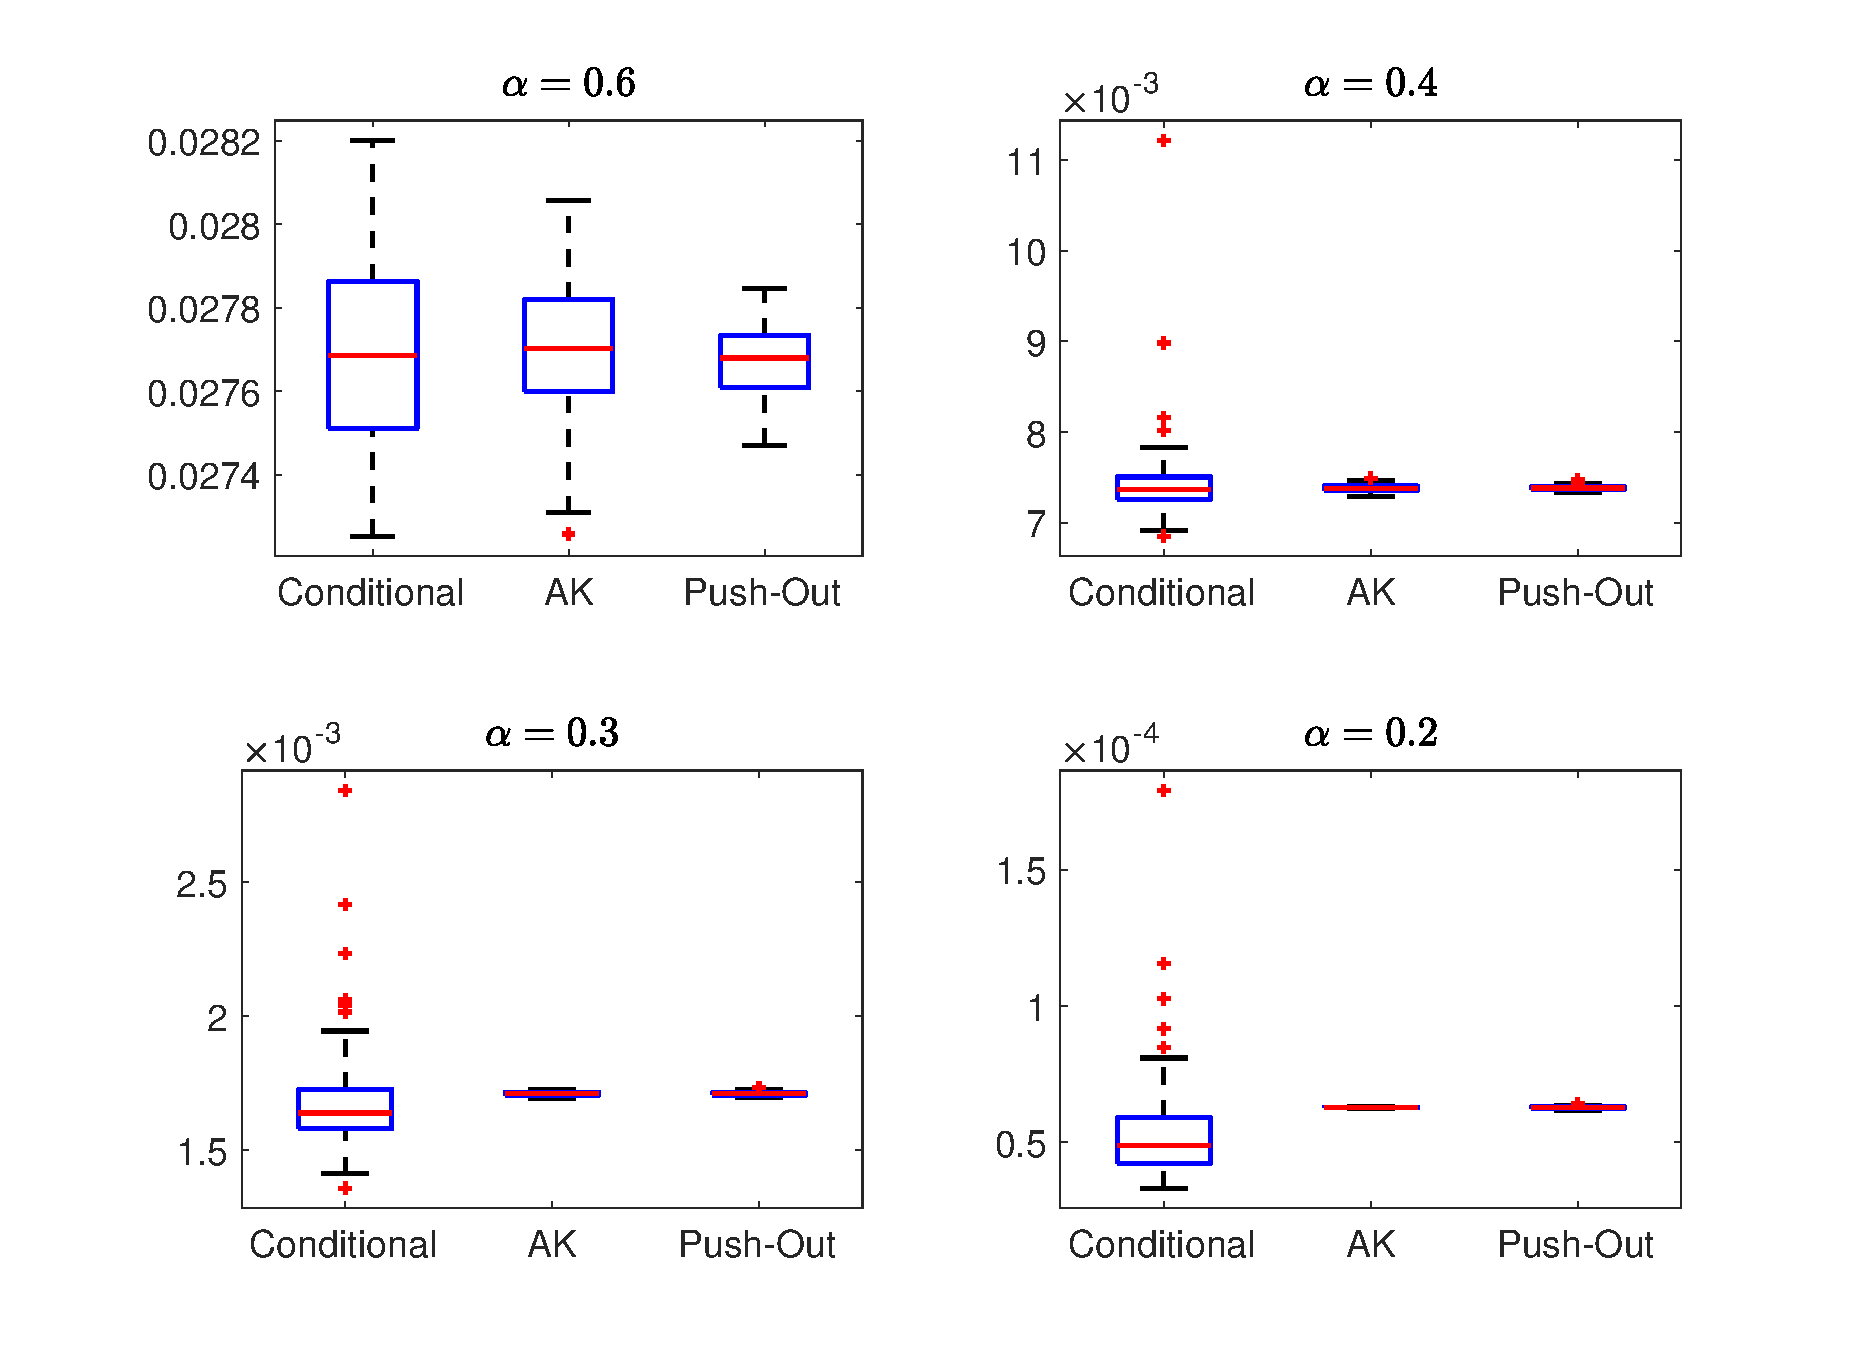
\includegraphics[width=1\textwidth]{skewdist.pdf}
    \caption{Results from $100$ runs, each with $R=10^5$ samples, of Conditional Monte Carlo, Asmussen Kroese, and our proposed method, for 30 iid $\sf{Weibull}(\alpha,1)$ rv's for varying shape parameter $\alpha$. We estimate the pdf at $s = \bb E[S] = 30 \,\Gamma(1+(1/\alpha))$ in each case.}

		\label{fig:weibull}
\end{figure} 


\section{Conclusion} \label{sec:Conclusion}
We have introduced a novel ``push-out'' Monte Carlo estimator for the unbiased estimation of the pdf of sums of random variables, and given several examples of its implementation.  The numerical experiments suggest that in terms of WNRV the proposed push-out estimator is preferable to the existing competitors (Conditional Monte Carlo, Asmussen-Kroese, and kernel density estimators). The main reason for this is that typically the evaluation of the gradient of the joint pdf 
$f_{\v X}$ is faster to compute than the conditional pdfs of $f_{\v X}$.
On the other hand, a shortcoming of our proposed estimator is that verifying the theoretical finiteness of its variance is difficult. In particular, in our numerical experiments we have implicitly assumed the moment condition $\Exp \big| \v{X} \cdot \nabla \log f_{\v{X}}(\v{X})\big|^4<\infty$.

% \section*{Acknowledgments}
% Robert Salomone and Patrick Laub have been supported by the Australian Research Council Centre of Excellence for
% Mathematical \& Statistical Frontiers (ACEMS), under grant number CE140100049. Zdravko Botev has been supported by the Australian Research Council grant DE140100993.   We thank Liam Hodgkinson for helpful suggestions in the early stages of this work. 

% \section*{References}
% \bibliographystyle{model1b-num-names}
% \bibliography{pdfEstimation}


\begin{subappendices}

\section{Proofs}


\begin{proof}[Proposition~\ref{prop:DensityRepresentation}]

Define the cdf $F_S(s) =\int_{\v 1 \cdot \v x \le s} f_{\v{X}}(\v{x}) \dd \v{x} \,,$
so that the pdf is
$
f_S(s) =\frac{\dd}{\dd s}  F_S(s)
$.
The change of variables  $\v x = s \v y$ yields:
\[
 F_S(s)=\int_{\mathcal{R}_s} f_{\v{X}}(s \v{y}) |s|^n \dd \v{y}\quad s\not =0, 
\]
where the notation $\int_{\mathcal{R}_s}$ means $\int_{\v{1}\cdot\v{y}\le 1}$ if $s >0$, else $\int_{\v{1}\cdot\v{y}> 1}$ for $s<0$.

Let $\varphi(s):=\int_{\mathcal{R}_s}\frac{\dd}{\dd s} \left( f_{\v{X}}(s \v{y})  |s|^n\right)\dd \v{y} $. We will use the fact 
that $\varphi(s)=f_S(s)$ almost everywhere (i.e.\ except possibly on sets of zero Lebesgue measure) on $s\not\in(-\epsilon,\epsilon)$ for an arbitrarily small $\epsilon>0$. 


In order to justify  the identity $\varphi(s)=f_S(s)$
(almost everywhere) in the case of 
$s>\epsilon$ (similar arguments apply for $s<\epsilon$),
we use the Fubini-Tonelli theorem for exchanging the order of
integration. This exchange 
holds under the integrability condition 
\begin{equation}
\label{integrability}
\int_\epsilon^s\int_{\v{1}\cdot\v{y}\le 1}\left|\frac{\dd}{\dd t} \left( f_{\v{X}}(t \v{y})  t^n\right)\right|\dd \v{y}\dd t<\infty
\end{equation}
and the existence of a continuous $\nabla f_{\v X}$, both of which follow from  Assumption~\ref{assumption} (verified at the end of this proof). Using the Fubini-Tonelli theorem \cite{rosenthal2006first} we then write:
\[
\begin{split}
\int_\epsilon^s\varphi(t)\dd t&=\int_\epsilon^s\int_{\v{1}\cdot\v{y}\le 1}\frac{\dd}{\dd t} \left( f_{\v{X}}(t \v{y})  t^n\right)\dd \v{y}\dd t\\
&=\int_{\v{1}\cdot\v{y}\le 1}\int_\epsilon^s\frac{\dd}{\dd t} \left( f_{\v{X}}(t \v{y})  t^n\right)\dd t\dd \v{y}\\
&=\int_{\v{1}\cdot\v{y}\le 1} ( f_{\v{X}}(s \v{y})  s^n -
 f_{\v{X}}(\epsilon \v{y})  \epsilon^n)\dd \v{y}=F_S(s)-F_S(\epsilon)
\end{split}
\]
Hence, by the fundamental theorem of Calculus,   $\varphi$ equals the  derivative of $F_S$ up to a set of measure zero. 
In other words, $\varphi(s)=f_S(s),s>\epsilon$ almost everywhere. 



To proceed, we write $\sign(x)= x / |x| = \frac{\dd}{\dd x} |x|$
\begin{align*}
f_S(s)=\varphi(s) &=\int_{\mathcal{R}_s} |s|^n \v{y} \cdot \nabla f_{\v{X}}(s \v{y}) + n |s|^{n-1} \sign(s) f_{\v{X}}(s \v y)  \dd \v{y} \\
&=\textstyle\int_{\mathcal{R}_s} \left[ \v{y} \cdot \nabla \log f_{\v{X}}(s \v{y}) + \frac{n \, \sign(s)}{|s|} \right] |s|^{n} f_{\v{X}}(s \v y)  \dd \v{y} ,
\end{align*}
so after a change of variables $\v{y} = \v{x} / s$ and using $\sign(x)/|x|=1/x$, we obtain
\begin{align*}
f_S(s)
&= \int_{\v 1 \cdot \v x \le s } \big[ \frac{\v{x}}{s} \cdot \nabla \log f_{\v{X}}(\v{x}) + \frac{n}{s} \big] f_{\v{X}}(\v x)  \dd \v{x}
= \frac{1}{s} \Exp \big\{ \ind{ \v 1 \cdot \v X \le s } [ \v{X} \cdot \nabla \log f_{\v{X}}(\v{X}) + n ] \big\} \,.
\end{align*}
To verify \eqref{integrability}, note that after using the change of variable above, it can be upper bounded by
\[
\textstyle\int_\epsilon^s\frac{1}{t} \Exp \big\{ \ind{ \v 1 \cdot \v X \le t }| \v{X} \cdot \nabla \log f_{\v{X}}(\v{X}) + n |\big\} \dd t\leq (\Exp \big| \v{X} \cdot \nabla \log f_{\v{X}}(\v{X})\big | + n) \int_\epsilon^s\frac{1}{t}\dd t<\infty,
\]
which is bounded by assumption. 
\end{proof}

\begin{proof}[Corollary~\ref{cor:WeightedSums}]
Consider $\widetilde{\v{X}} := \v c \v X$, with density
$f_{\widetilde{\v{X}}}(\widetilde{\v{x}}) = f_{\v X}(\v{c}^{-1} \widetilde{\v{x}} ) / | \prod_{i=1}^n c_i |$.
As $\v{X}$ satisfies Assumption~\ref{assumption} then so does $\widetilde{\v{X}}$, so we apply Proposition~\ref{prop:DensityRepresentation} to $\widetilde{\v{X}}$ to get
\begin{align*}
f_S(s) 
&= \frac{1}{s} \Exp_{f_{\widetilde{\v{X}}}}\big\{ \ind{\v{1} \cdot \widetilde{\v{X}} \le s} [ \widetilde{\v{X}} \cdot \nabla \log f_{\widetilde{\v{X}}}(\widetilde{\v{X}}) + n ] \big\} = \frac{1}{s} \Exp_{f_{\v{X}}}\big\{ \ind{\v{c} \cdot \v{X} \le s} [ \v{X} \cdot \nabla \log f_{\v{X}}(\v{X}) + n ] \big\}, 
\end{align*}
where the second equality uses
$\nabla \log f_{\widetilde{\v{X}}}(\widetilde{\v{x}}) 
= \v{c}^{-1} \nabla \log f_{\v X}(\v{c}^{-1} \widetilde{\v{x}} )  $.
\end{proof}

\begin{proof}[Proposition~\ref{lemma:MarginalDensity}]
Note that the marginal density of $X_i$ can be written as
 \[ f_{X_i}(s)
    =\int_{x_{-i} \in \RL^{n-1}} \frac{\dd}{\dd s}  \int_{x_i \le s} f_{\v{X}}(\v{x}) \dd x_i \dd \v{x}_{-i}.
 \]
 Applying the same push-out technique (now using the change of variables $x_1 = s y_1$) as in Proposition~\ref{prop:DensityRepresentation} for the inner integral, and then rearranging yields
 \begin{align*}
    f_{X_i}(s)
    &=\frac1s \int_{\RL^{n}} \ind{x_i \le s} (x_i \nabla_i \log f_{\v{X}}(\v{x}) + 1 )  f_{\v{X}}(\v{x}) \dd \v{x} 
    = \frac1s \Exp \big\{ \ind{ X_i \le s} [ \big(X_i \nabla_i \log f_{\v X}(\v{X}) + 1 \big) ] \big\} \,.
    \end{align*}

\end{proof}



\end{subappendices}